\documentclass[UTF8,a4paper,12pt]{ctexart}

\usepackage{geometry}
\geometry{left=2.6cm,right=2.6cm,top=2.5cm,bottom=2.5cm}
\usepackage{amsmath,amssymb,bm}
\usepackage{graphicx}
\usepackage{booktabs}
\usepackage{array}
\usepackage{float}
\usepackage{caption}
\usepackage{subcaption}
\usepackage{enumitem}
\usepackage{hyperref}
\usepackage{xcolor}
\usepackage{longtable}

\graphicspath{{figures/}}
\hypersetup{
  colorlinks=true,
  linkcolor=black,
  citecolor=black,
  urlcolor=blue
}
\captionsetup{font=small,labelfont=bf}
\setlist[itemize]{leftmargin=2em}
\setlist[enumerate]{leftmargin=2em}

\newcommand{\ud}{\,\mathrm{d}}
\newcommand{\um}{\ensuremath{\mu\mathrm{m}}}
\newcommand{\cmone}{\ensuremath{\mathrm{cm}^{-1}}}

\title{\heiti 基于稳健性诊断与介电函数约束 TMM 的\\碳化硅外延层厚度反演研究}
\author{蔡文傑\quad 陈翔\quad 单夕航}
\date{2026 年 7 月 7 日}

\begin{document}
\maketitle

\begin{abstract}
碳化硅外延层厚度是外延片质量评估和器件制备中的关键几何参数。红外反射谱中的干涉条纹携带厚度信息，但实际反演会受到折射率色散、材料吸收、多光束干涉、入射角、载流子相关介电响应以及数据预处理口径的共同影响。若只使用相邻峰距公式，容易把局部极值识别误差和简化折射率假设误认为厚度结论；若直接使用复杂全谱拟合模型，又可能因参数非唯一性得到缺乏可解释性的低误差结果。

针对同一块 SiC 晶圆片在 $10^\circ$ 与 $15^\circ$ 入射角下的红外反射谱，本文建立了从数据稳健性诊断、频域主周期提取、峰谷级次差法（FOD）基线、色散修正、Dong2012 介电函数约束转移矩阵法（TMM）、残差诊断到波段权重稳健性分析的递进式反演流程。多种预处理方法均给出全波段主周期 $\Delta\nu=250\ \cmone$，滑窗 FFT 得到 $\Delta\nu\in[244.537,256.000]\ \cmone$，说明反射谱中存在稳定条纹尺度。基于 Dong/TMM 的双角度联合拟合显示，厚度低谷稳定处于 $7.4\text{--}7.6\ \um$ 附近；在受 $\nu_p$ 物理边界约束的局部细化中，代表点为 $d^\ast=7.465\ \um$，联合 RMSE 为 $0.00171152$。进一步改变波段权重后，最优厚度仅在 $7.465\text{--}7.485\ \um$ 内移动，最大位移为 $0.020\ \um$。收尾阶段新增最终证据一致性审计，将 Dong/TMM 双角度分算、参数敏感性、局部优化、bootstrap 和波段权重证据统一到同一厚度轴上；纳入最终判断的强证据覆盖约为 $7.400\text{--}7.580\ \um$。因此，本文将 $d\approx7.4\text{--}7.6\ \um$ 作为当前证据下的最强候选区间，并将 $d^\ast=7.465\ \um$ 作为受约束 Dong/TMM 模型下的代表值。

\textbf{关键词：} 碳化硅外延层；红外反射谱；FFT；FOD；转移矩阵法；介电函数；残差诊断；稳健性分析
\end{abstract}

\section{问题重述}

碳化硅（SiC）是典型的第三代半导体材料。外延层厚度会影响器件击穿电压、导通电阻和工艺一致性，因此需要可靠的非破坏性测量方法。红外反射法利用外延层上下界面反射光之间的干涉条纹反演厚度，具有非接触、速度快、适合晶圆级检测等优点。

本文处理的核心数据为同一块 SiC 外延片在两个入射角下的红外反射率谱。记入射角为 $\theta\in\{10^\circ,15^\circ\}$，观测数据为
\begin{equation}
\mathcal D_\theta=
\{(\nu_i,R_{\mathrm{obs},\theta}(\nu_i))\}_{i=1}^{N_\theta},
\end{equation}
其中 $\nu_i$ 为波数，单位为 $\cmone$，$R_{\mathrm{obs},\theta}$ 为实验反射率。目标是在没有外部真值厚度的条件下，根据两组反射谱确定 SiC 外延层厚度，并说明结论的可信程度。

该问题的难点不只是写出峰距公式，而是判断公式和模型是否真的被数据支撑。红外条纹的周期、振幅和相位会同时受到折射率、消光系数、载流子浓度、材料吸收、多光束干涉、入射角和仪器基线影响。因此，本文将问题拆成三层：
\begin{enumerate}
  \item 数据层：确认反射谱中是否存在稳定的厚度相关条纹周期；
  \item 模型层：建立能够解释色散、吸收和多光束干涉的物理反演模型；
  \item 评价层：通过双角度一致性、参数敏感性、残差诊断和波段权重分析检验厚度结论。
\end{enumerate}

\section{模型假设与符号说明}

\subsection{模型假设}

结合题目数据形态和红外干涉测厚原理，本文采用如下假设。

\begin{enumerate}
  \item 外延层与衬底界面在测量区域内近似平行，厚度可用单一标量 $d$ 表示。该假设是条纹法测厚的基本几何前提。
  \item 附件 1 与附件 2 来自同一块 SiC 晶圆片，因此 $10^\circ$ 与 $15^\circ$ 反演出的厚度应在误差范围内一致。若两角度明显分离，说明模型或数据处理存在未闭合因素。
  \item 外延层与衬底存在可观测光学差异，使反射谱对外延层厚度具有可识别性。若二者光学性质完全相同，单层膜厚度对反射谱的影响会显著减弱。
  \item FOD 和 FFT 只用于提取条纹周期与厚度初值，不作为最终厚度结论。最终厚度以包含复折射率和多光束干涉的 TMM 模型为主。
  \item Dong2012 介电函数参数可作为 4H-SiC 红外响应的物理约束来源，但其参数来自文献样品，不能直接视为本题样品真实材料参数。
  \item 为吸收仪器尺度和基线差异，全谱拟合允许实验反射率与模型反射率之间存在仿射校准：
  \begin{equation}
  R_{\mathrm{obs}}(\nu)\approx aR_{\mathrm{model}}(\nu;d)+b.
  \end{equation}
\end{enumerate}

\subsection{符号说明}

\begin{table}[H]
\centering
\caption{主要符号说明}
\begin{tabular}{lll}
\toprule
符号 & 含义 & 单位或说明\\
\midrule
$\nu$ & 波数 & $\cmone$\\
$\lambda_0$ & 真空波长 & $\um$\\
$d$ & 外延层厚度 & $\um$\\
$\theta_0$ & 空气中入射角 & $^\circ$\\
$\theta_1$ & 外延层内折射角 & Snell 定律给出\\
$n(\nu)$ & 折射率实部 & 色散函数\\
$k(\nu)$ & 消光系数 & 色散函数\\
$\tilde n(\nu)$ & 复折射率 & $n(\nu)+ik(\nu)$\\
$R_{\mathrm{obs}}$ & 实验反射率 & 观测数据\\
$R_{\mathrm{model}}$ & 模型反射率 & TMM 计算结果\\
$\Delta\nu$ & 条纹周期 & $\cmone$\\
$\nu_p$ & 等离子体频率参数 & Dong 介电函数参数\\
$\gamma$ & Drude 阻尼 & Dong 介电函数参数\\
$\Gamma_L,\Gamma_T$ & 声子阻尼 & 纵、横光学声子阻尼\\
$\mathrm{RMSE}$ & 均方根误差 & 反射率尺度\\
\bottomrule
\end{tabular}
\end{table}

\section{数据预处理与条纹周期诊断}

\subsection{数据统一}

题目数据以波数为横坐标。波数与真空波长满足
\begin{equation}
\lambda_0(\um)=\frac{10000}{\nu(\cmone)}.
\end{equation}
该式中的 $10000$ 来自 $\mathrm{cm}$ 与 $\um$ 的单位换算，是后续厚度公式中必须保留的因子。若反射率以百分数给出，则统一转换为 $R=R_{\%}/100$。为进行 FFT 分析，对排序后的原始数据插值到等间隔波数网格：
\begin{equation}
R_{\mathrm{grid}}(\nu_j)=
\mathrm{interp}\left(\nu_j;\nu_{\mathrm{raw}},R_{\mathrm{raw}}\right).
\end{equation}

图 \ref{fig:raw} 展示了双角度原始谱线。两组数据均有明显振荡条纹，说明反射谱中存在厚度相关周期结构；同时，局部强吸收、背景起伏和角度差异也提示不能仅用单个峰距作为最终结论。

\begin{figure}[H]
\centering
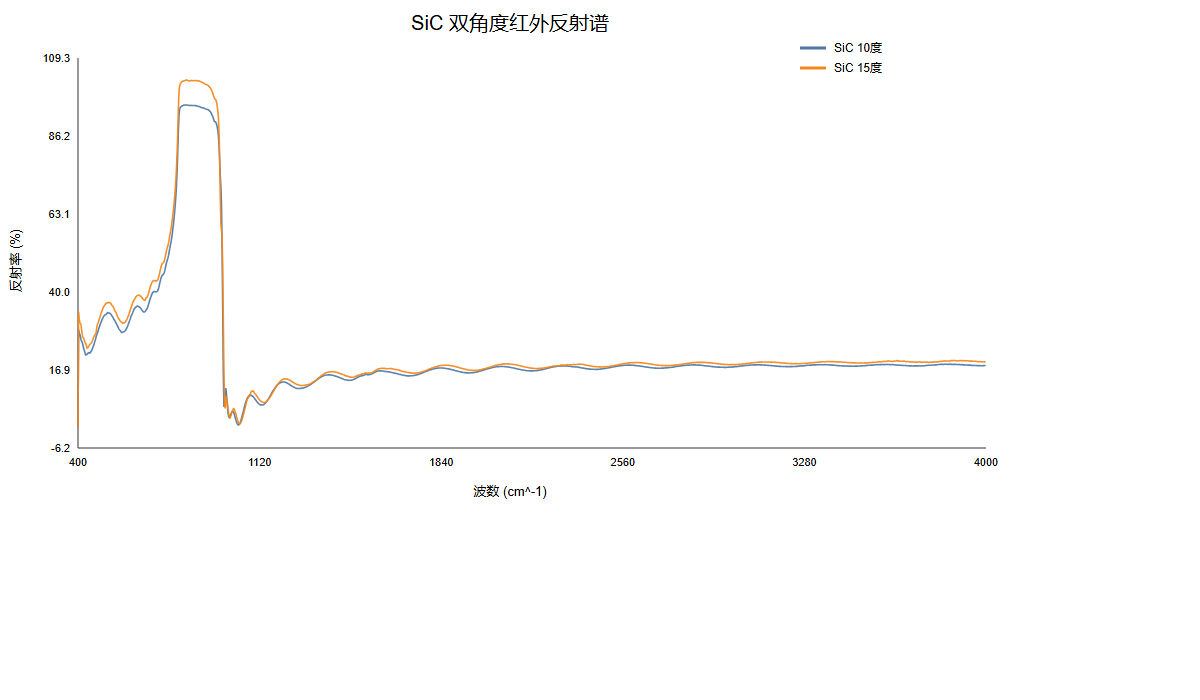
\includegraphics[width=0.92\textwidth]{paper_fig00_sic_dual_angle_raw.png}
\caption{SiC 双角度原始红外反射谱}
\label{fig:raw}
\end{figure}

\subsection{预处理稳健性}

为避免某一预处理方式主导结论，本文比较了去均值中心化、移动平均去趋势、多项式去趋势、滚动中位数基线、滚动分位数基线和一阶差分等方法。不同预处理的作用不同：去均值保留原始形态，移动平均和多项式去趋势削弱慢变背景，滚动中位数和分位数基线提高对异常点的稳健性，一阶差分则突出局部变化率。

实验结果显示，上述预处理均给出一致的全波段主周期：
\begin{equation}
\Delta\nu=250\ \cmone.
\end{equation}
这一结果说明，主周期不是某一种预处理制造出的偶然结构，而是反射谱中稳定存在的信息。图 \ref{fig:fft} 展示了不同预处理下的频域厚度初值。

\begin{figure}[H]
\centering
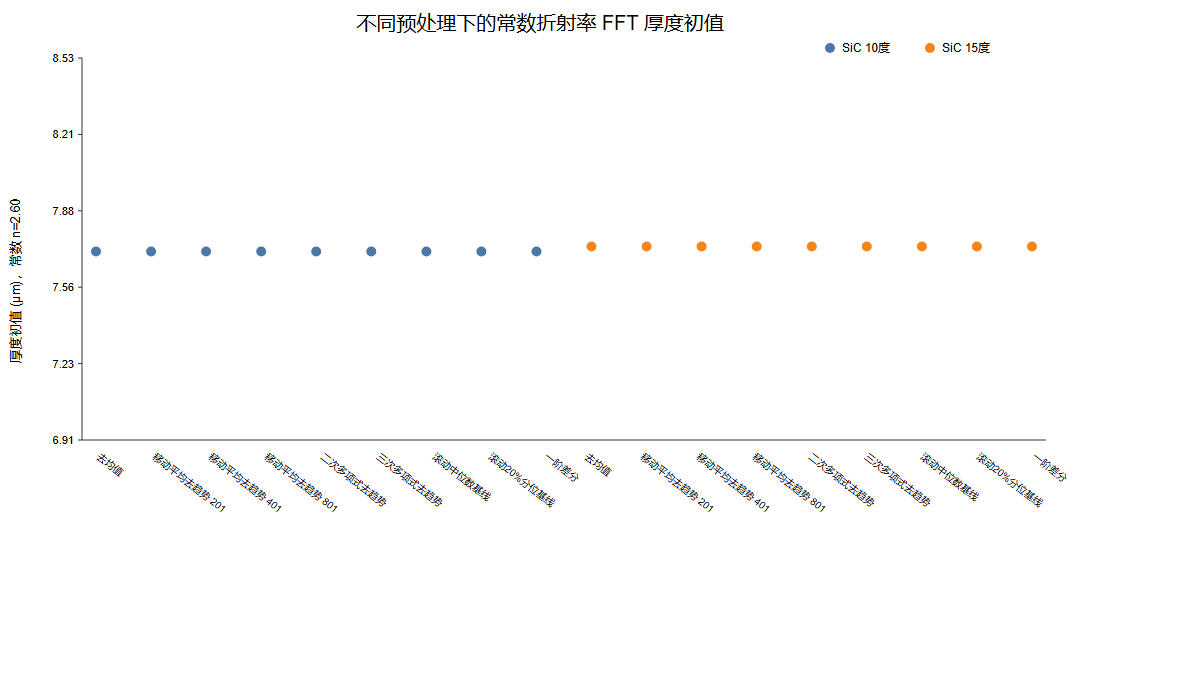
\includegraphics[width=0.88\textwidth]{data_processing_fft_thickness_seed.png}
\caption{不同预处理方法下的 FFT 厚度初值}
\label{fig:fft}
\end{figure}

进一步采用滑窗 FFT 检查局部波段稳定性。本文取窗口宽度 $1200\ \cmone$，步长 $250\ \cmone$。滑窗结果为
\begin{equation}
\Delta\nu\in[244.537,256.000]\ \cmone.
\end{equation}
在常数 $n=2.60$ 口径下，对应厚度初值约为
\begin{equation}
d_{\mathrm{FFT}}\in[7.529,7.882]\ \um.
\end{equation}
图 \ref{fig:sliding} 显示，局部窗口主周期集中于 $250\ \cmone$ 附近。由此可得数据层结论：反射谱中存在稳定条纹尺度，但将该尺度换算为真实厚度仍依赖折射率和物理模型。

\begin{figure}[H]
\centering
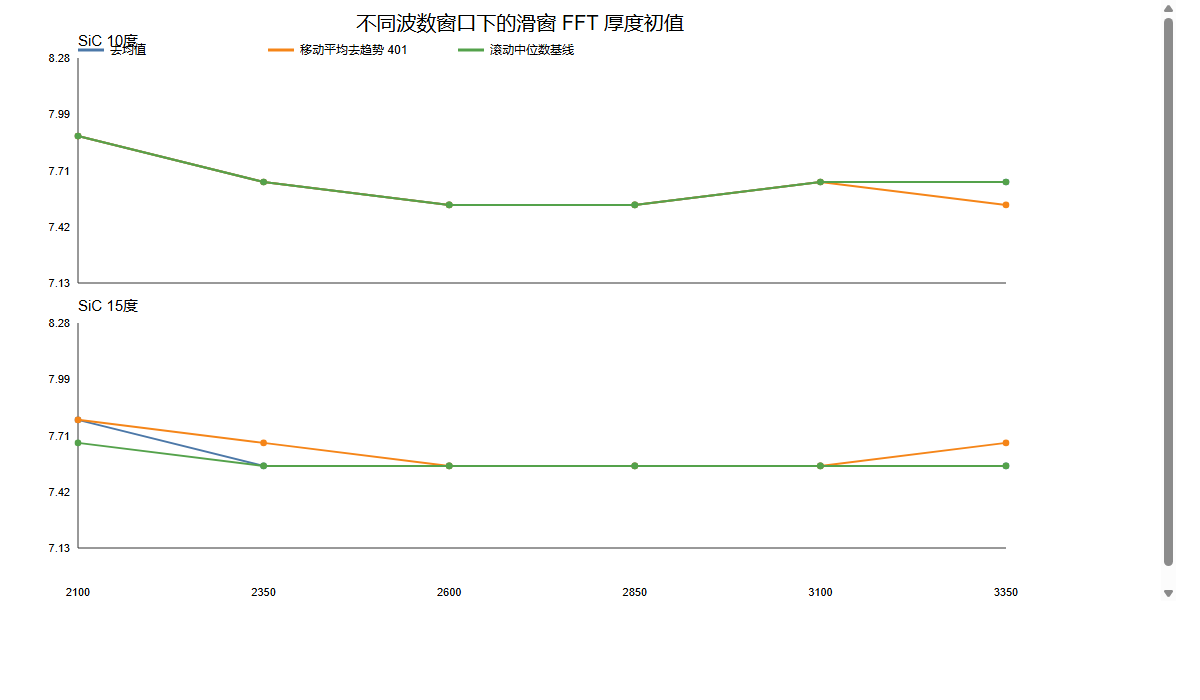
\includegraphics[width=0.88\textwidth]{sliding_fft_thickness_by_window.png}
\caption{滑窗 FFT 主周期与厚度初值}
\label{fig:sliding}
\end{figure}

\section{基线模型：峰距法与 FOD}

\subsection{相邻峰距公式}

薄膜上下界面反射光在外延层中形成往返光程差。在忽略吸收和复杂反射相位时，光程差近似为
\begin{equation}
\Delta L=2dn\cos\theta_1.
\end{equation}
由 Snell 定律，若空气折射率近似为 1，则
\begin{equation}
\cos\theta_1=
\sqrt{1-\left(\frac{\sin\theta_0}{n}\right)^2}.
\end{equation}
相邻同类极值的级次差近似为 1，因此有
\begin{equation}
1\approx
\frac{2dn\cos\theta_1\Delta\nu}{10000}.
\end{equation}
解得常用峰距公式：
\begin{equation}
d\approx
\frac{10000}{2n\cos\theta_1\Delta\nu}.
\label{eq:spacing}
\end{equation}

式 \eqref{eq:spacing} 物理意义清晰，但假设较强：折射率在局部近似常数，极值识别可靠，反射相位不随波段变化，且忽略吸收和多光束干涉。因此，本文仅将峰距法作为透明基线。

\subsection{FOD 多极值拟合}

单个峰距只使用两个极值点，容易受到噪声和局部吸收影响。FOD（fringe order difference）方法使用多个同类极值相对参考极值的级次差进行拟合。设同类极值序列为 $\nu_0,\nu_1,\ldots,\nu_q$，取最高波数极值为参考点 $\nu_{\mathrm{ref}}=\nu_q$，定义
\begin{equation}
\Delta m_i=q-i.
\end{equation}
若折射率近似常数，则有
\begin{equation}
\Delta m_i\approx
\frac{2dn\cos\theta_1}{10000}
(\nu_{\mathrm{ref}}-\nu_i).
\end{equation}
通过最小二乘估计 $d$，可降低单个峰距误差对结果的影响。

本文同时尝试色散 FOD，将常数 $n$ 替换为 $n(\nu)$，并定义
\begin{equation}
g(\nu)=n(\nu)\nu\cos\theta_1(\nu),
\end{equation}
则级次差关系写为
\begin{equation}
\Delta m_i\approx
\frac{2d}{10000}
\left[g(\nu_{\mathrm{ref}})-g(\nu_i)\right].
\end{equation}
FOD 和色散 FOD 的结果说明：条纹周期确实携带厚度信息，但不同折射率模型会显著改变厚度数值。因此，最终模型必须引入更完整的材料介电函数和全谱反射模型。

\section{介电函数约束 TMM 模型}

\subsection{复折射率与相位厚度}

SiC 在红外波段具有明显色散和吸收，外延层与衬底还可能因载流子浓度不同而具有不同介电响应。令复折射率为
\begin{equation}
\tilde n(\nu)=n(\nu)+ik(\nu)=\sqrt{\varepsilon(\nu)}.
\end{equation}
外延层内相位厚度为
\begin{equation}
\delta(\nu,d)=
\frac{2\pi}{\lambda_0}
\tilde n_1(\nu)d\cos\theta_1(\nu).
\end{equation}
对于空气--外延层--衬底结构，单层膜反射振幅可写为 Airy 形式：
\begin{equation}
r(\nu,d)=
\frac{r_{01}+r_{12}\exp(2i\delta)}
{1+r_{01}r_{12}\exp(2i\delta)}.
\end{equation}
模型反射率为
\begin{equation}
R_{\mathrm{model}}(\nu,d)=|r(\nu,d)|^2.
\end{equation}

本文基于 Dong et al. 对 4H-SiC 红外介电响应的 Lorentz--Drude 型建模思想，引入 $\nu_p$、$\gamma$、$\Gamma_L$、$\Gamma_T$ 等参数，以描述声子共振和载流子贡献。由于题目未给出本样品掺杂浓度，本文不把这些参数完全自由化，而采用文献参数附近的缩放敏感性与物理边界约束。

\subsection{双角度联合目标函数}

为同时利用 $10^\circ$ 与 $15^\circ$ 数据，本文以双角度联合 RMSE 为目标函数。对每个角度先允许仿射校准
\begin{equation}
R_{\mathrm{obs},\theta}(\nu)
\approx
a_\theta R_{\mathrm{model},\theta}(\nu;d)+b_\theta,
\end{equation}
再计算联合误差：
\begin{equation}
\mathrm{RMSE}_{\mathrm{joint}}
=
\sqrt{
\frac{1}{N_{10}+N_{15}}
\sum_{\theta\in\{10^\circ,15^\circ\}}
\sum_i
\left[
a_\theta R_{\mathrm{model},\theta}(\nu_i;d)+b_\theta
-R_{\mathrm{obs},\theta}(\nu_i)
\right]^2}.
\label{eq:rmse}
\end{equation}

与只看单角度误差相比，式 \eqref{eq:rmse} 能检查同一块晶圆片在不同入射角下是否给出一致厚度。若两个角度低谷相距很远，即使联合 RMSE 较低，也需要谨慎解释。

\subsection{\texorpdfstring{$\nu_p$}{nu\_p} 物理边界}

等离子体频率 $\nu_p$ 与载流子浓度相关。为避免模型将 $\nu_p$ 当作纯数学调参量，本文将其缩放范围限制为
\begin{equation}
s_{\nu_p,\mathrm{epi}}\in[0.75,1.75],
\qquad
s_{\nu_p,\mathrm{sub}}\in[0.75,1.25].
\end{equation}
对应的载流子浓度量级约为
\begin{equation}
N_{\mathrm{epi}}\approx
9.20\times10^{16}\text{--}5.01\times10^{17}\ \mathrm{cm^{-3}},
\end{equation}
\begin{equation}
N_{\mathrm{sub}}\approx
2.45\times10^{18}\text{--}6.81\times10^{18}\ \mathrm{cm^{-3}}.
\end{equation}
这些数值仅作为优化边界，不代表本文已经测得样品真实掺杂浓度。

\section{模型求解与结果分析}

\subsection{TMM 拟合结果}

在受 $\nu_p$ 边界约束的 Dong/TMM 局部细化中，双角度联合代表点为
\begin{equation}
d^\ast=7.465\ \um,\qquad
\mathrm{RMSE}_{\mathrm{joint}}=0.00171152.
\end{equation}
分角度看，$10^\circ$ 单独最佳厚度为 $7.490\ \um$，$15^\circ$ 单独最佳厚度为 $7.430\ \um$。两个角度并不完全重合，但均落在 $7.4\text{--}7.6\ \um$ 附近。图 \ref{fig:fit} 展示了代表点下的双角度拟合曲线。

\begin{figure}[H]
\centering
\begin{subfigure}{0.48\textwidth}
\centering
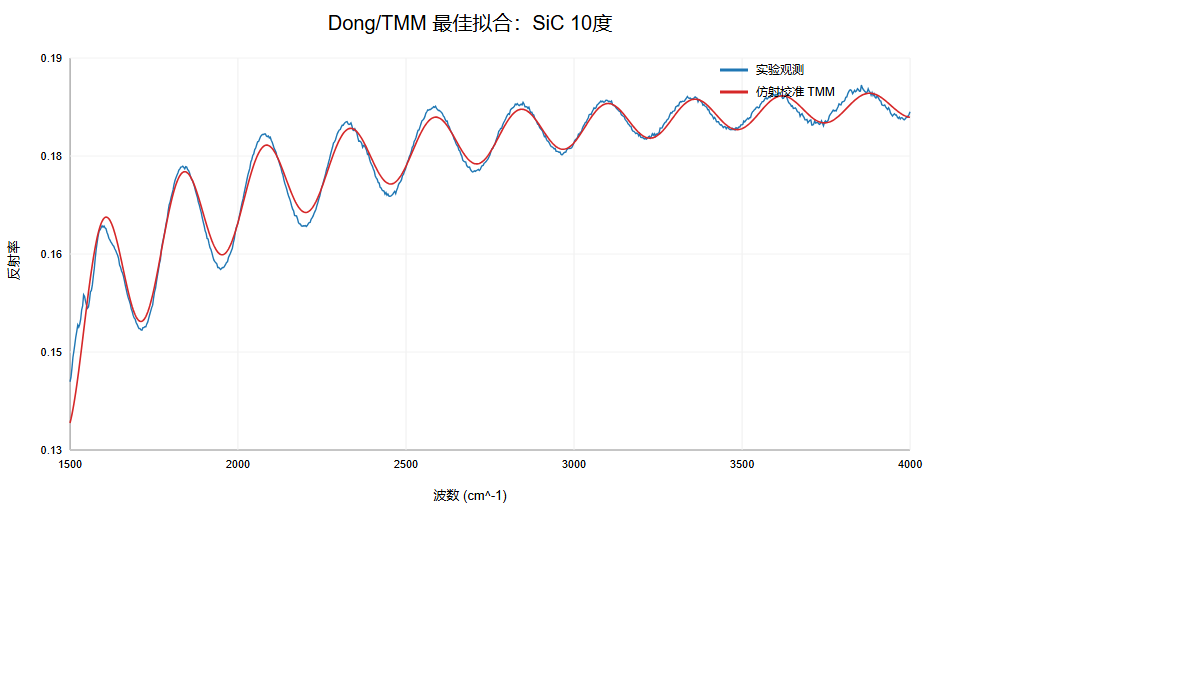
\includegraphics[width=\textwidth]{paper_fig05_tmm_bestfit_SiC_10deg.png}
\caption{$10^\circ$ 入射角}
\end{subfigure}
\hfill
\begin{subfigure}{0.48\textwidth}
\centering
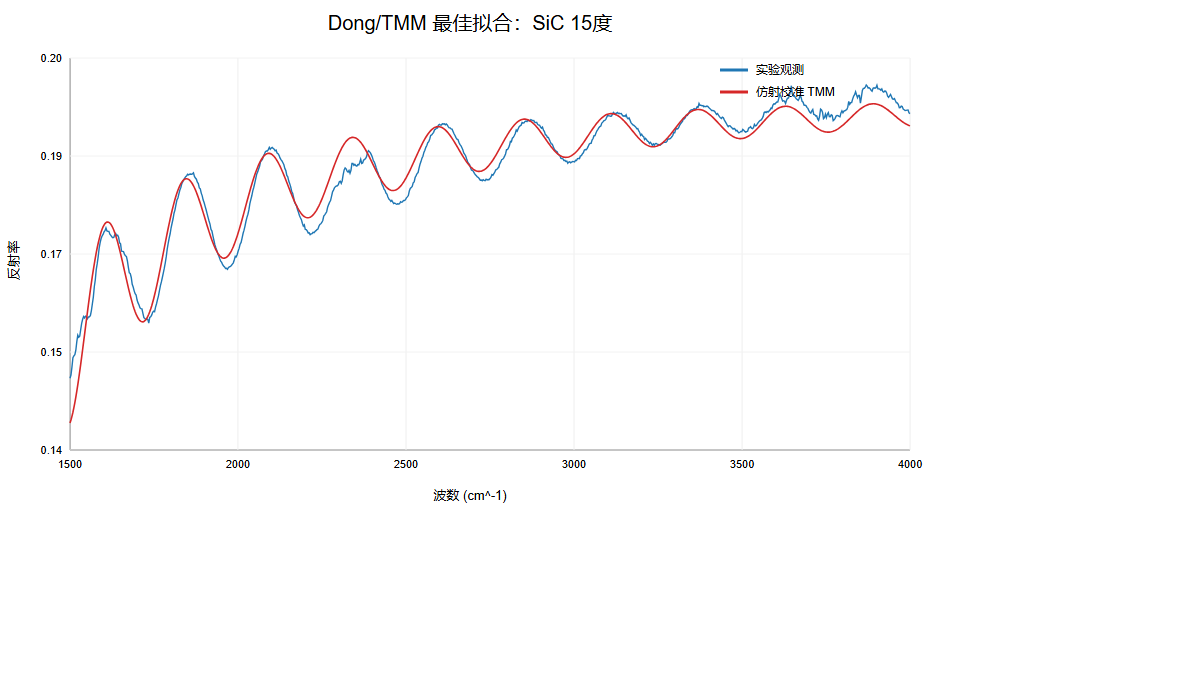
\includegraphics[width=\textwidth]{paper_fig05_tmm_bestfit_SiC_15deg.png}
\caption{$15^\circ$ 入射角}
\end{subfigure}
\caption{受约束 Dong/TMM 代表点下的双角度拟合结果}
\label{fig:fit}
\end{figure}

\subsection{参数敏感性}

为检查厚度低谷是否依赖单一参数组合，本文对 $\nu_p$、$\gamma$、$\Gamma_L$、$\Gamma_T$ 和波段选择进行了多组敏感性实验。表 \ref{tab:routes} 汇总了主要路线的厚度结果。

\begin{table}[H]
\centering
\caption{主要模型路线与厚度结果}
\label{tab:routes}
\begin{tabular}{p{0.38\textwidth}p{0.25\textwidth}p{0.23\textwidth}}
\toprule
模型路线 & 厚度结果 / \um & 说明\\
\midrule
常数折射率 FOD，$10^\circ$ & $7.191\pm0.148$ & 基线模型，角度一致性不足\\
常数折射率 FOD，$15^\circ$ & $6.603\pm0.089$ & 基线模型，受折射率假设影响\\
Dong2012 表 2 介电函数 TMM，$10^\circ$ & $7.460$ & 中高候选\\
Dong2012 表 2 介电函数 TMM，$15^\circ$ & $7.400$ & 中高候选\\
Dong/TMM $\nu_p$ 敏感性 & $7.440\text{--}7.580$ & 当前最强候选来源\\
Dong/TMM $\gamma$ 敏感性 & $7.440\text{--}7.460$ & 稳健性补充\\
Dong/TMM 声子阻尼敏感性 & $7.400\text{--}7.480$ & 稳健性补充\\
有 $\nu_p$ 边界局部细化 & $7.455\text{--}7.465$ & 代表点 $7.465$\\
固定参数残差块 bootstrap & 中位数 $7.455$ & 固定材料参数下的不确定性检查\\
\bottomrule
\end{tabular}
\end{table}

$\nu_p$ 敏感性热力图如图 \ref{fig:nup} 所示。厚度低谷主要集中在 $7.4\text{--}7.6\ \um$ 附近，但外延层 $\nu_p$ 在受约束局部细化中触及上界，说明材料参数识别尚未完全闭合。

\begin{figure}[H]
\centering
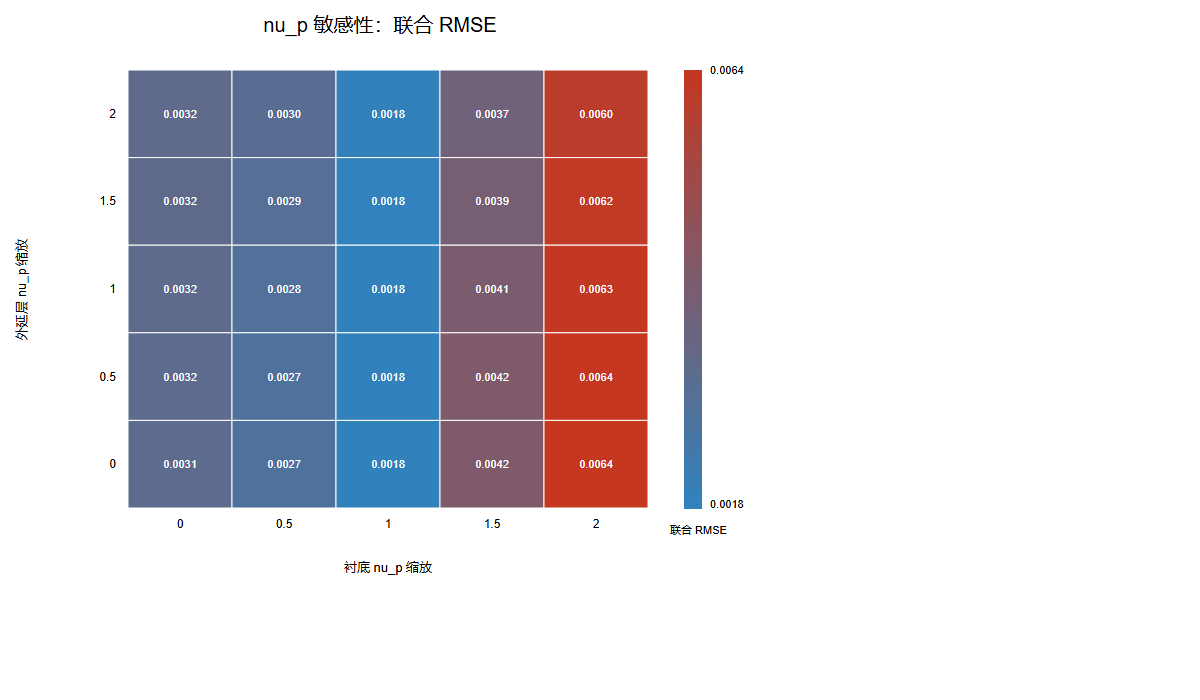
\includegraphics[width=0.82\textwidth]{paper_fig10_rmse_heatmap_nu_p_sensitivity.png}
\caption{$\nu_p$ 缩放参数下的联合 RMSE 热力图}
\label{fig:nup}
\end{figure}

\subsection{残差诊断}

仅有低 RMSE 不足以证明模型可信，因为复杂模型可能在局部参数组合下拟合出错误厚度。本文进一步检查残差结构。结果显示，$10^\circ$ 数据的 RMSE 为 $0.00131074$，残差一阶自相关为 $0.9726$；$15^\circ$ 数据的 RMSE 为 $0.00211230$，残差一阶自相关为 $0.9834$。这说明残差不是独立白噪声，而是存在连续结构，尤其 $15^\circ$ 更明显。

\begin{figure}[H]
\centering
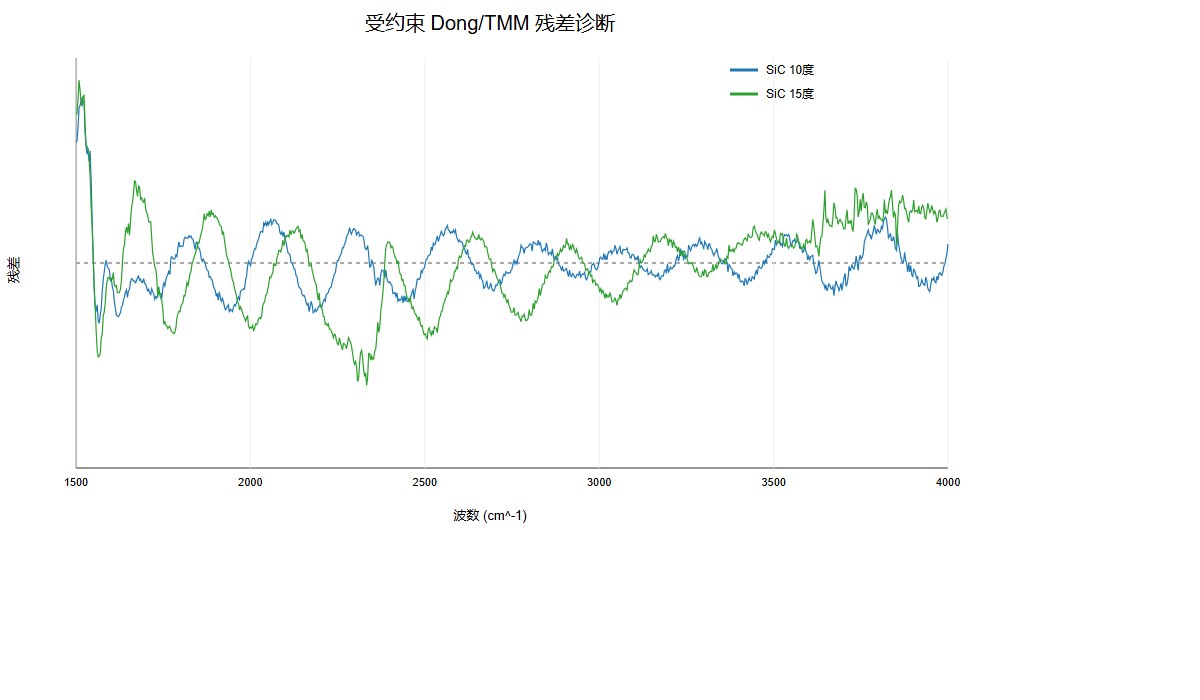
\includegraphics[width=0.88\textwidth]{residual_diagnostics_angle_residuals.png}
\caption{双角度 TMM 残差曲线}
\label{fig:residual}
\end{figure}

残差诊断的意义在于提醒我们：当前模型能够定位厚度低谷，但还没有完全解释全部谱线细节。因此，本文将 $7.465\ \um$ 写为代表点，而不是无条件最终认证厚度。

\section{稳健性分析与最终结论}

\subsection{波段权重稳健性}

红外谱不同波段的物理信息量不同，部分吸收区或低信噪比区可能影响拟合。为检查厚度是否由少数异常波段支撑，本文固定当前受约束 Dong/TMM 参数，只改变波段权重。四种权重口径下，最优厚度位于
\begin{equation}
d^\ast\in[7.465,7.485]\ \um,
\end{equation}
相对全波段等权口径最大位移为
\begin{equation}
\Delta d_{\max}=0.020\ \um.
\end{equation}

\begin{figure}[H]
\centering
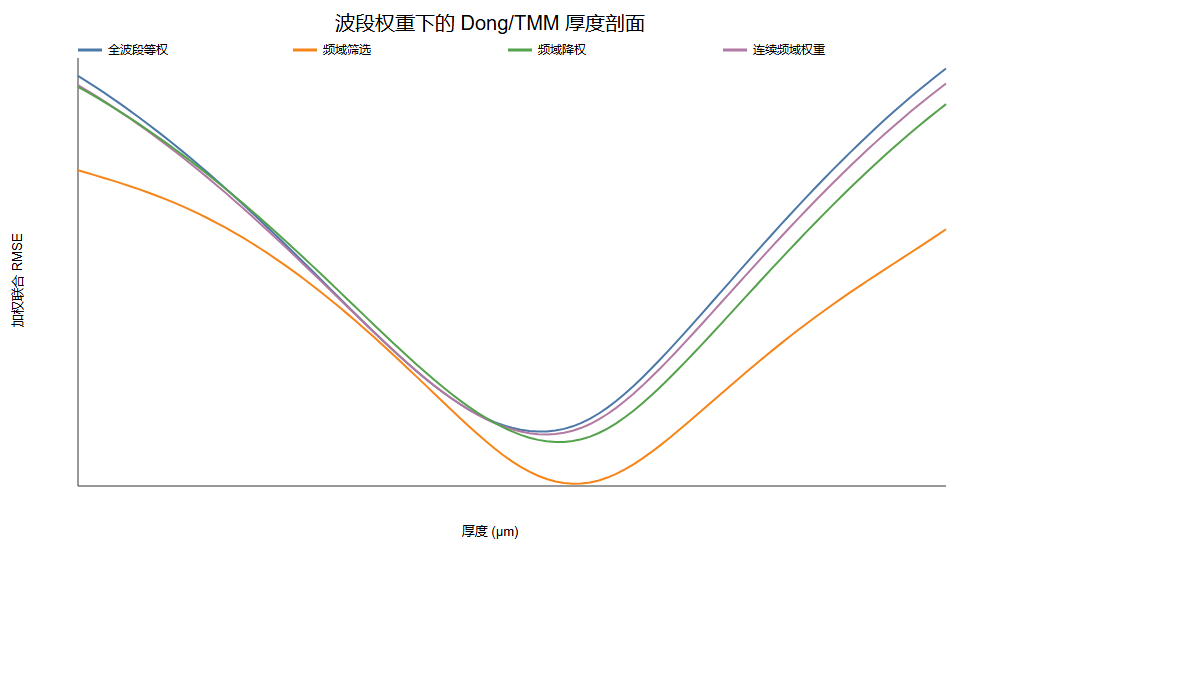
\includegraphics[width=0.82\textwidth]{band_weighted_tmm_profile.png}
\caption{波段权重变化下的 TMM 厚度剖面}
\label{fig:band}
\end{figure}

固定材料参数下的 RMSE--厚度剖面如图 \ref{fig:profile} 所示。低谷位于 $7.455\text{--}7.465\ \um$ 附近，说明在当前参数条件下厚度低谷清晰。

\begin{figure}[H]
\centering
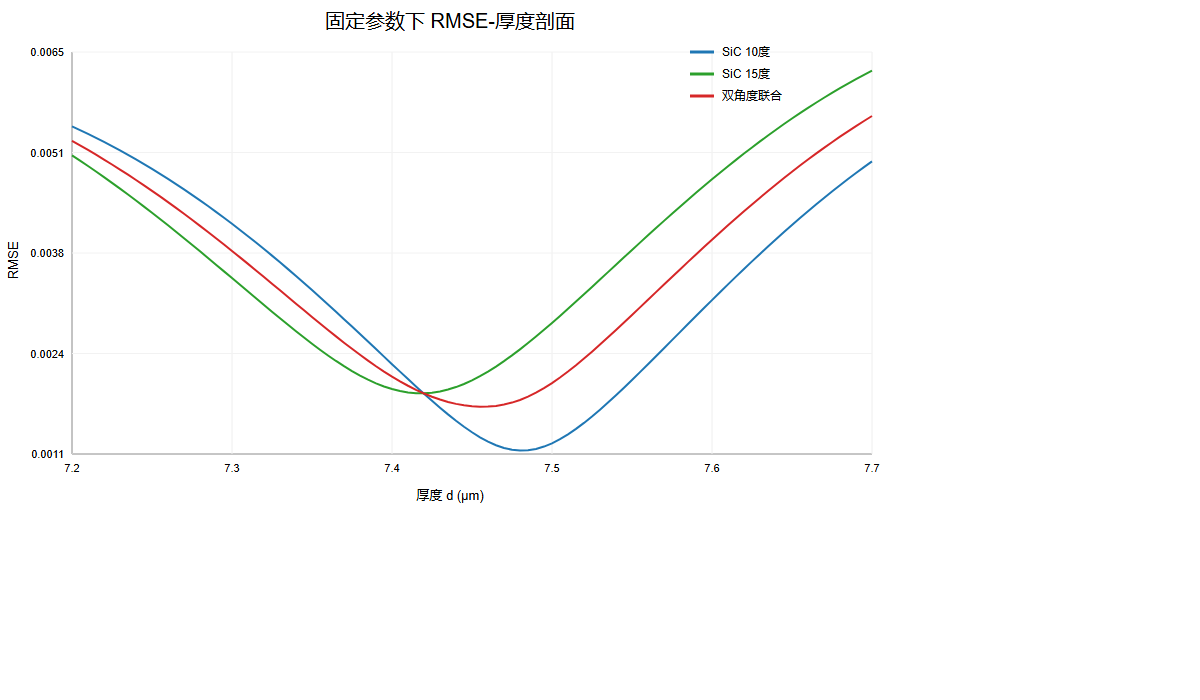
\includegraphics[width=0.82\textwidth]{paper_fig02_tmm_profile.png}
\caption{固定参数下的 TMM 厚度 RMSE 剖面}
\label{fig:profile}
\end{figure}

\subsection{最终证据一致性审计}

为了避免最终结论依赖散落脚本或单一调参结果，本文在收尾阶段新增最终证据一致性审计。该审计只读取已经生成并有文件记录的实验结果，不重新调参，不扩大搜索，也不把 FFT 或 FOD 的初值伪装成最终厚度。其核心思想是把不同证据放到同一厚度轴上，检查它们是否共同指向同一区间。

图 \ref{fig:finalaudit} 汇总了纳入最终判断的证据。Dong2012 表 2 介电函数 TMM 双角度分算给出 $7.400\text{--}7.460\ \um$；$\nu_p$ 敏感性给出 $7.440\text{--}7.580\ \um$；$\gamma$、声子阻尼、波段选择、受物理边界约束的局部细化、固定参数 bootstrap 与波段权重剖面均没有把低谷推出 $7.4\text{--}7.6\ \um$ 的范围。因而，最终论文不再追求把厚度写成过度精确的单点，而采用“稳健区间 + 代表点”的表达。

\begin{figure}[H]
\centering
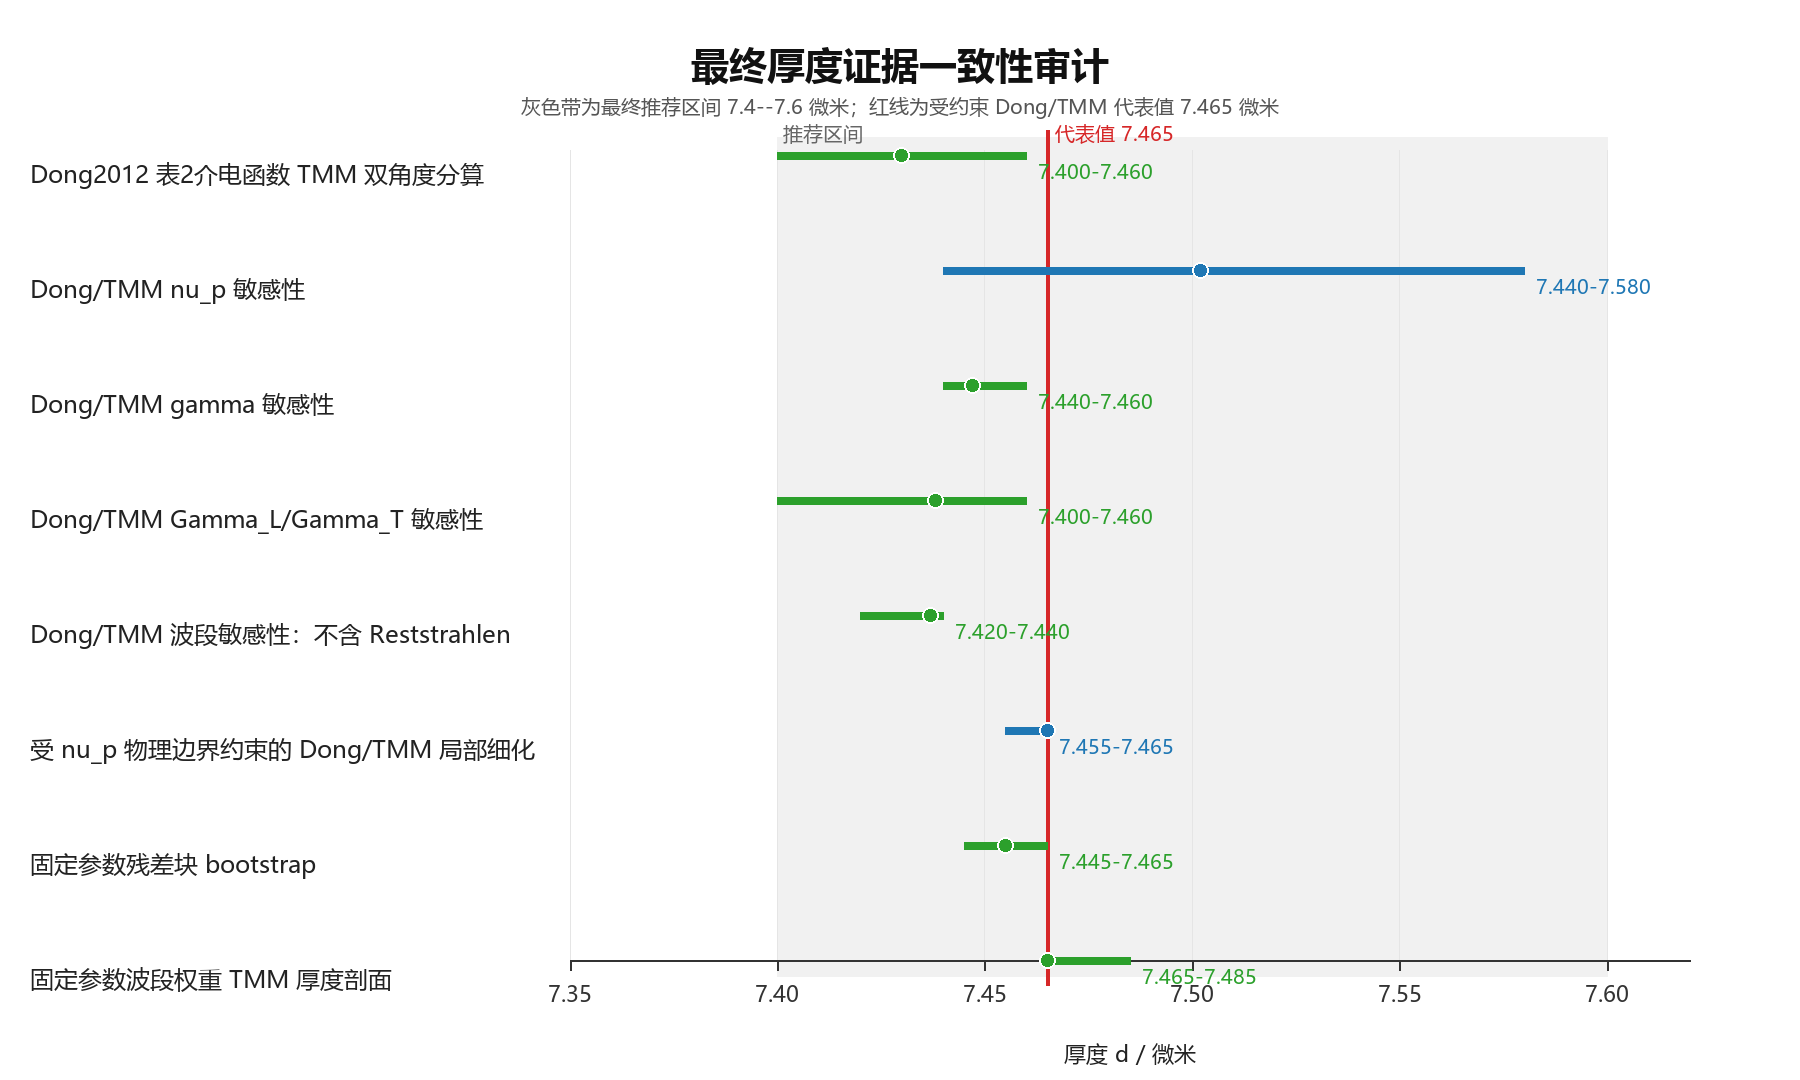
\includegraphics[width=0.98\textwidth]{final_evidence_audit.png}
\caption{最终厚度证据一致性审计}
\label{fig:finalaudit}
\end{figure}

\subsection{结果汇总}

\begin{table}[H]
\centering
\caption{关键结果汇总}
\label{tab:summary}
\begin{tabular}{lll}
\toprule
项目 & 结果 & 解释\\
\midrule
全波段 FFT 主周期 & $250\ \cmone$ & 多预处理一致\\
滑窗 FFT 主周期 & $[244.537,256.000]\ \cmone$ & 局部周期稳定\\
受约束 Dong/TMM 代表点 & $7.465\ \um$ & 当前主模型代表值\\
双角度联合 RMSE & $0.00171152$ & 主模型误差\\
$10^\circ$ 单角度最佳厚度 & $7.490\ \um$ & 与联合结果接近\\
$15^\circ$ 单角度最佳厚度 & $7.430\ \um$ & 残差更明显\\
波段权重稳健范围 & $[7.465,7.485]\ \um$ & 稳健性旁证\\
最终证据审计覆盖 & $[7.400,7.580]\ \um$ & 强证据合并范围\\
推荐候选区间 & $7.4\text{--}7.6\ \um$ & 当前最稳妥结论\\
\bottomrule
\end{tabular}
\end{table}

综合数据处理、FOD/FFT 初值、Dong/TMM 全谱拟合、参数敏感性、残差诊断、波段权重分析和最终证据一致性审计，本文认为 SiC 外延层厚度的当前最强候选区间为
\begin{equation}
\boxed{
d\approx7.4\text{--}7.6\ \um
}.
\end{equation}
若需要给出单一代表值，则在受 $\nu_p$ 物理边界约束的 Dong/TMM 局部细化条件下，可写为
\begin{equation}
\boxed{
d^\ast=7.465\ \um
}.
\end{equation}
但该代表值不应被解释为完整物理置信区间中心，因为材料参数不确定性尚未完全传播。

\section{模型评价与改进方向}

本文的主要优点如下。第一，先用多种预处理和滑窗 FFT 证明条纹周期是稳定数据事实，再进入物理模型，避免直接调参。第二，FOD、FFT 和 TMM 形成递进关系：FOD 与 FFT 提供可解释初值，TMM 负责解释复折射率、吸收和多光束干涉。第三，双角度联合拟合利用了同一晶圆片厚度一致性的约束。第四，参数敏感性、残差自相关和波段权重分析共同构成了结果可信度检验。

模型仍有不足。第一，Dong2012 介电函数参数来自文献样品，迁移到本题样品时存在材料差异。第二，$\gamma$ 与 $\Gamma_L,\Gamma_T$ 的物理边界尚未完全建立。第三，外延层 $s_{\nu_p}$ 在受约束优化中触及上界，说明材料参数识别不充分。第四，$15^\circ$ 残差自相关较高，提示偏振、各向异性、局部吸收区或仪器基线仍可能影响拟合。

后续改进可从三方面展开：一是进一步精读近年关于 epi-wafer 红外测厚、VMD-LSP 频域提取和全局优化反演的文献；二是补充 $\gamma$、$\Gamma_L,\Gamma_T$ 与材料物性的边界关系；三是在算力允许时进行全局优化或贝叶斯不确定性传播，以检查局部低谷是否仍保持稳定。

\section{参考文献}

\begin{enumerate}[label={[\arabic*]}]
  \item Li Zhi-Yun, Sun Ji-Wei, Zhang Yu-Ming, Zhang Yi-Men, Tang Xiao-Yan. Methods for Thickness Determination of SiC Homoepilayers by Using Infrared Reflectance Spectroscopy. \textit{Chinese Physics Letters}, 2010, 27(6): 068103. DOI: 10.1088/0256-307X/27/6/068103.
  \item Dong Lin, Sun Guo-Sheng, Liu Zheng, Liu Xing-Fang, Zhang Feng, Yan Guo-Guo, Zhao Wan-Shun, Wang Lei, Li Xi-Guang, Wang Zhan-Guo. Characterization of 4H-SiC substrates and epilayers by Fourier transform infrared reflectance spectroscopy. \textit{Chinese Physics B}, 2012, 21(4): 047802. DOI: 10.1088/1674-1056/21/4/047802.
  \item Oishi Shingo, Hijikata Yasuto, Yaguchi Hiroyuki, Yoshida Sadafumi. Simultaneous Determination of Carrier Concentration, Mobility, and Thickness of SiC Homoepilayers by Infrared Reflectance Spectroscopy. \textit{Japanese Journal of Applied Physics}, 2006, 45(12L): L1226. DOI: 10.1143/JJAP.45.L1226.
  \item Troparevsky M. Claudia, Sabau Adrian S., Lupini Andrew R., Zhang Zhenyu. Transfer-matrix formalism for the calculation of optical response in multilayer systems: from coherent to incoherent interference. \textit{Optics Express}, 2010, 18(24): 24715. DOI: 10.1364/OE.18.024715.
  \item Sun Jiaxing, Li Zhisong, Zhang Haojie, Song Jinlong, Zhai Tianbao. An improved method for measuring epi-wafer thickness based on the infrared interference principle: Addressing interference quality and multiple interferences in double-layer structures. \textit{Results in Physics}, 2023, 54: 107146. DOI: 10.1016/j.rinp.2023.107146.
  \item Dutta Rajdeep, Tian Siyu Isaac Parker, Liu Zhe, Lakshminarayanan Madhavkrishnan, Venkataraj Selvaraj, Cheng Yuanhang, Bash Daniil, Chellappan Vijila, Buonassisi Tonio, Senthilnath Jayavelu. Extracting film thickness and optical constants from spectrophotometric data by evolutionary optimization. \textit{PLOS ONE}, 2022, 17(11): e0276555. DOI: 10.1371/journal.pone.0276555.
  \item Chahal J., Rahbany N., El-Helou Y., Wu K. T., Bruyant A., Zgheib C., Kazan M. Temperature dependence of the anisotropy of the infrared dielectric properties and phonon-plasmon coupling in n-doped 4H-SiC. \textit{Journal of Physics and Chemistry of Solids}, 2024, 187: 111861. DOI: 10.1016/j.jpcs.2023.111861.
  \item Polyanskiy Mikhail N. Refractiveindex.info database of optical constants. \textit{Scientific Data}, 2024, 11: 94. DOI: 10.1038/s41597-023-02898-2.
  \item Byrnes Steven J. \textit{tmm: transfer matrix method Python package}. GitHub repository: \url{https://github.com/sbyrnes321/tmm}.
\end{enumerate}

\appendix
\section{附录：程序与图表来源}

本文数值结果均来自项目内 Python 脚本和输出文件。主要脚本包括：
\begin{itemize}
  \item \texttt{data\_processing\_diagnostics.py}：多预处理 FFT 稳健性；
  \item \texttt{sliding\_fft\_diagnostics.py}：滑窗 FFT 周期稳定性；
  \item \texttt{dong2012\_tmm\_constrained\_refinement.py}：受 $\nu_p$ 边界约束的 Dong/TMM 局部细化；
  \item \texttt{residual\_diagnostics.py}：分角度残差和残差自相关；
  \item \texttt{band\_weighted\_tmm\_profile.py}：波段权重稳健性分析；
  \item \texttt{final\_evidence\_audit.py}：最终证据审计表和厚度一致性图；
  \item \texttt{paper\_assets.py} 与 \texttt{manuscript\_visual\_assets.py}：论文图表生成。
\end{itemize}

主要输出位于项目 \texttt{Experiments/outputs/}，图表位于 \texttt{Experiments/figures/}。本文提交版使用的 PNG 图由已有 SVG 图表转换得到，不改变实验数值。

\end{document}
